\documentclass{article}
\usepackage[utf8]{inputenc}
\usepackage{xcolor}
\pagestyle{myheadings} %this command changes the styling to have the page numbers on the top right 
\usepackage{listings}
\usepackage{tcolorbox}
\usepackage{blindtext}
\usepackage{textcomp}
\usepackage{amsmath}
\usepackage{float} % For fixing table and figures at their place
\usepackage{multirow} %For multiple rows in one column compared to other
\usepackage{color}   %May be necessary if you want to color links
\usepackage{hyperref}
\hypersetup{
    colorlinks=true, %set true if you want colored links
    linktoc=all,     %set to all if you want both sections and subsections linked
    linkcolor=blue,  %choose some color if you want links to stand out
}

\definecolor{light-gray}{gray}{0.95}
\definecolor{codegreen}{rgb}{0,0.6,0}
\definecolor{codegray}{rgb}{0.5,0.5,0.5}
\definecolor{codepurple}{rgb}{0.58,0,0.82}
\definecolor{backcolour}{rgb}{0.95,0.95,0.92}
\lstdefinestyle{mystyle}{
    backgroundcolor=\color{backcolour},   
    commentstyle=\color{codegreen},
    keywordstyle=\color{magenta},
    numberstyle=\tiny\color{codegray},
    stringstyle=\color{codepurple},
    basicstyle=\ttfamily\footnotesize,
    breakatwhitespace=false,         
    breaklines=true,                 
    captionpos=b,                    
    keepspaces=true,                 
    numbers=left,                    
    numbersep=5pt,                  
    showspaces=false,                
    showstringspaces=false,
    showtabs=false,                  
    tabsize=2
}
\lstset{style=mystyle,literate={~} {$\sim$}{1}}
\newcommand{\code}[1]{\colorbox{light-gray}{\texttt{#1}}}




\title{\vspace*{4cm}\textbf{Software Requirement Specification for Seminar and Talks Management System\vspace*{0.4cm}\\Team 33\vspace*{0.2cm}}}
\author{Jatin Tarachandani \\\small{CS20BTECH11021} \and Prashanth Sriram S \\\small{CS20BTECH11039}   \and Shambhu Kavir \\\small{CS20BTECH11045} \and Taha Adeel Mohammed \\\small{CS20BTECH11052} \vspace*{0.4cm} }

\date{\today}


\begin{document}

\maketitle



\newpage

\tableofcontents

\newpage

\section{Introduction}

\subsection{Definitions and Acronyms}
\begin{itemize}
    % \item SEE IF WE NEED ANYTHING HERE, LIKE IF WE COME UP WITH AN ACRONYM FOR THE APP
    \item SeTMaS: Seminar and Talks Management System, the name of the application
    \item IITH: Indian Institute of Technology Hyderabad
    \item Talk: Any Seminar or Webinar or Event that needs to be booked on a particular venue and for a particular time duration.
    % define superadmin
    \item Super Admin: An admin who is granted elevated privileges over the other admins of the system. These privileges include adding and removing admin privileges from other users, transferring his status as super admin to another admin. Addition and removal of other admins can only be done by the super admin. 
\end{itemize}

\subsection{Purpose of this application}
This application is a seminar/talk booking management system: where faculty and students alike can place requests to book certain rooms at certain times to conduct talks and seminars, and a centralized platform for the administration governing these bookings to view requests, and accept and reject them as appropriate. This application  is also proposed to be integrated into the IITH mailing system, as described in the appendix below. 

This requirement specification is meant to serve as a guideline for what functionality is supported within this project; and what use cases are fulfilled by the app. 

\subsection{Scope of the application}
The functionalities fulfilled by this application are: 
\begin{itemize}
    \item Faculty/students/other IITH people will be able to submit requests to book one of the available rooms for a specific length of time as per their convenience. These requests will be approved by a governing authority consisting of approved administrators. 
    \item Said approved administrators will be able to view all the pending requests for booking, and be able to accept and reject them based on the content, time and date of the requester. 
    \item Even without login, any user will be able to view a calendar which displays all the upcoming seminars/talks along with their details. 
    \item This system will also be integrated with the IITH mailing system, with emails being sent to concerned parties when requests are made, accepted, and rejected. This system is elaborated on in \hyperref[mail_appendix]{Appendix 4.1}.%(INSERT APPENDIX HERE)
\end{itemize}

\subsection{Overview of this SRS}
The next few sections of this SRS talk about the use cases of the application. These range from things like installation, to making a request for a seminar, to the admin functionality of approving or denying requests for seminars. 
\\
Section 2 discusses the various users of the application, and tabulates all the use cases which are supported by the application. There are also some assumptions and constraints taken into account when planning the requirements for this software, which are also specified in section 2.
\\ 
Section 3 is an elaboration on every use case tabulated in section 2. It would consist of details like primary actors, preconditions, and main and alternate scenarios. Design constraints and processes that we thought of are also specified in this section. The appendices in section 4 deal with the UI and the IITH mailing integration.

\section{Description}
\subsection{Product Perspective}
  %May have to rephrase a bit
    SeTMaS is aimed towards a person who wants to book seminars as well as view the schedule of the seminars in the IITH campus. SeTMaS is intended to be a web-app that will run on any modern browser on any device. SeTMaS should be user-friendly, intuitive to use and be a reliable application.
\subsection{Product Functions}
The use cases supported by SeTMaS are shown in Table 1. 
\begin{table}[!htbp]
\footnotesize
\caption{Product Functions: Use Cases}
\begin{center}
\begin{tabular}{|c|c|p{0.35\linewidth}|}
    \hline
    \multirow{1}{0.35\linewidth}{\textbf{Class of use cases}}&\textbf{Use cases}&\textbf{Description of use cases}\\
    \hline
    \multirow{2}{0.35\linewidth}{Use cases related to Authorization}&\hyperref[uclogin]{Login}&Login into SeTMaS using google sign in with IITH id \\
    \hline
    \multirow{2}{0.35\linewidth}{Use Cases related to Publishing Info}&\hyperref[ucdisplaycalendar]{Display Calendar}&Display the calendar with all the accepted seminars\\
    \hline
    \multirow{17}{0.35\linewidth}{Use Cases related to Booking a Slot}&\hyperref[ucrequestbooking]{Request Booking}&Users can request a room for a time duration \\
    \cline{2-3}
    &\hyperref[ucviewmybookings]{View My Bookings}&Users can view all the booking requests they have made and see the status of them\\
    \cline{2-3}
    &\hyperref[uccancelpendingrequest]{Cancel Pending Request}&Users can cancel their own pending request\\
    \cline{2-3}
    &\hyperref[ucviewbookingrequests]{View Booking Requests}&A logged-in valid admin can view all the booking requests made by users in a user-friendly view\\
    \cline{2-3}
    &\hyperref[ucapprovebookingrequests]{Approve Booking Request}&A logged-in valid admin can approve a booking request raised by a user\\
    \cline{2-3}
    &\hyperref[ucrejectbookingrequests]{Reject Booking Request}&A logged-in valid admin can reject a booking request raised by a user\\
    \cline{2-3}
    &\hyperref[uccancelapprovedrequest]{Cancel Approved Request}&A logged-in valid admin can cancel an approved request\\
    \hline
    \multirow{3}{0.35\linewidth}{Use cases related to Admin Management}
    &\hyperref[ucviewadminslist]{View Admins list}& Any admin can view the list of all the existing admins\\
    \cline{2-3}
    &\hyperref[ucaddanadmin]{Add an Admin}&The super-admin can add a user to the admin list\\
    \cline{2-3}
    &\hyperref[ucremoveanadmin]{Remove an Admin}&The super-admin can remove an admin from the admin list\\
    \cline{2-3}
    &\hyperref[uctransfersuperadminrole]{Transfer Super-Admin role}&The super-admin can transfer their role to another admin\\
    \hline
    \multirow{16}{0.35\linewidth}{Use cases related to Mailing Notifications}&\hyperref[ucbookingrequestconfirmation]{Booking request confirmation}&A mail should be sent to the user confirming that the request has been made\\
    \cline{2-3}
    &\hyperref[ucbookingapprovalnotification]{Booking Approval notification}&A mail should be sent to the user conveying that the booking is approved\\
    \cline{2-3}
    &\hyperref[ucbookingrejectionnotification]{Booking Rejection notification}&A mail should be sent to the user conveying that the booking is rejected\\
    \cline{2-3}
    &\hyperref[ucseminarnotification]{Seminar Notification}&Mails should be sent to those subscribed notifying them of the booked seminar\\
    \cline{2-3}
    &\hyperref[ucseminarreminder]{Seminar Reminder}&Mails should be sent to those subscribed reminding them of the upcoming seminars\\
    \cline{2-3}
    &\hyperref[ucseminarcancellationnotification]{Seminar Cancellation Notification}&Mails should be sent to those subscribed notifying them of the cancellation\\
    \hline
    % \multirow{3}{*}{Class1}&C1-Case1&Desc\\
    % \cline{2-3}
    % &C1-Case2&Desc\\
    % \cline{2-3}
    % &C1-Case3&Desc\\
    % \hline
    % \multirow{1}{*}{Class2}&Only Case&Desc\\
    % \hline
\end{tabular}
\end{center}
\label{tab:multicol}
\end{table}

\subsection{Principal Actors}
\begin{enumerate}
    \item \textbf{Guests:} be able to view the public calendar on the web-app
    \item \textbf{Users:} be able to log-in and book seminars/talks
    \item \textbf{Admin:} be able to Log-in and Approve/Reject booking requests.
    %%%%%%%%%%%%%%Admins can delete approved bookings?
    %%%%%%%%%%%%%%Admin can Blacklist users?
    \item \textbf{Superadmin:} be able to add or remove admins, may transfer the role of superadmin to another admin. There can only be one superadmin recognised by the system at a given time. 
    \item \textbf{system:} manages the back-end computations and sends out mail notifications as appropriate
\end{enumerate}
\subsection{Assumptions and Constraints}
\begin{enumerate}
    \item The full working of SeTMaS depends on a working internet connection and the running of the back-end server of SeTMaS.
    \item All the users will have a valid IITH email id to access the system.
    \item All the users will have access to a modern browser that can run JavaScript. %May need to be more specific with the version maybe? May need to provide examples of modern browsers?
    \item For an administrator to carry out administrative functions in the application, his IITH email ID must be registered as an admin by the super admin of the system. The details of this process are described in this document.  
\end{enumerate}

%structure of this document:
% - Intro : purpose, scope(here we'll replace with priorities), definitions if we need, references (mainly for UI), overview. - Jatin
% - description: perspective(here we will describe different kinds of users like admin and regular users aka principal actors), tabulation of the use case(IMP), assumptions and constraints(connectivity etc.) - Taha, Prashanth
% - specific requirements : this section will mainly consist of elaborating on each use case defined in the table in the previous section, performance(here we can just mention time guarantees), design constraints/things to keep in mind(can add a point about the mailing system), brief description of proposed UI. - Shambu, Jatin 
% - appendices for UI, one for describing the mailing integration with IITH mail, one sample usage of the software(someone wants to book a specific room at a specific time for XYZ seminar) alongside UI sketches or screenshots(see how feasible this is) - All 4 based on the content of the previous sections

\section{Specific Requirements and Use Cases}
 Here we describe the functional requirements of our application by elaborating on the various use cases given in the previous section. 
\subsection{Authorization Use Cases}
\textbf{Authorization/Login}: 
\label{uclogin}
\begin{itemize}
    \item \textit{Primary Actor}: User, or Admin, or Superadmin (hereafter in this use case referred to as 'client') 
    \item \textit{Precondition}: The client has access to their IITH Google account, and has a working connection to the internet. %see if this is enough
    \item \textit{Main Scenario}:
    \begin{enumerate}
        \item Client connects to the web application using a compatible browser. 
        \item Client clicks on the login button specified on the home page of the application. 
        \item Client is prompted to login using their Google account. The Google accounts shown to the client will be the ones they have logged in to on that browser, not necessarily just their IITH Google account. 
        \item Client logs in through Google using their required IITH account.
        \item The main authorized user screen of the application is displayed. 
    \end{enumerate}
    \item \textit{Alternate Scenario}:
        \begin{enumerate}
            \item Authentication fails. In this case, prompt the user that they have not used a valid IITH Google account to login, and provide a button to go back to the guest homepage. 
        \end{enumerate}
\end{itemize}

% suddenly writing
\subsection{Publishing Info Use Case}
\textbf{Display Calendar}:
\label{ucdisplaycalendar}
\begin{itemize}
    \item \textit{Primary Actor}: Any kind of client (Guest, User, Admin, Superadmin), needs no further credentials %changed this to include guest
    \item \textit{Precondition}: The client has a working connection to the internet.
    \item \textit{Main Scenario}: 
    \begin{enumerate}
        \item Client connects to the web application using a compatible browser.
        \item The calendar with all the upcoming seminars along with their details is displayed on the homepage.
        
    \end{enumerate}
    
\end{itemize}

% book book book
\subsection{Booking Slots Use Cases}
\textbf{Request Booking}
\label{ucrequestbooking}
\begin{itemize}
    \item \textit{Primary Actor}: Most often a normal authenticated user, however this functionality can be used by admins or superadmin. 
    \item \textit{Precondition}: The user should be logged in and authenticated using their IITH Google Account via the login process explained above. 
    \item \textit{Main Scenario}: 
    \begin{enumerate}
        \item Client initiates the slot booking process. 
        \item Client selects a date from the available selections.
        \item Client is prompted to enter the details of the seminar. This includes \begin{enumerate}
            \item Title
            \item Details
            \item The starting and ending time of the room booking
            \item The department
            \item The email ID of the requester
            \item List of the mailing lists, in which the notification and reminders are to be sent. Such as: seminar@cse.iith.ac.in, etc.
            \item List of time durations, before which reminder mails must be sent. Such as 30 minutes before, 24 hours before, etc.
        \end{enumerate}
        \item Assuming the aforementioned details are entered correctly, the request will be submitted.
        \item If the system registers the request, \hyperref[ucbookingrequestconfirmation]{A mail confirming the same} is sent to the client.
    \end{enumerate}
    \item \textit{Alternate Scenario}:
    \begin{enumerate}
        \item User enters an incorrect time (i.e.) a time that overlaps with a \textbf{confirmed} booking(this will be visible when selecting a date). In this case, an error popup will be seen when trying to create the request for room booking, and it will not go through to the system. 
        \item User enters an incorrect or infeasible time duration for the reminder, for example, greater than 72* hours, or when the time at which the reminder is to be sent precedes the time of the booking request. In this case, an error popup will be seen notifying the user of the same to correct it and it will not register as a successful request
        \item User enters too many time durations for the reminder, (greater than 6*) in which case, an error popup will be seen notifying the user of the same to correct it and it will not register as a successful request. This is done to prevent the spamming of reminder mails.
        %%%%%% * - I have currently used arbitrary numbers. Need to review
    \end{enumerate}
\end{itemize}

\textbf{View My Bookings}
\label{ucviewmybookings}
\begin{itemize}
    \item \textit{Primary Actor}: A user, admin, or superadmin, hereafter referred to in this case as client. 
    \item \textit{Precondition}: Must have successfully logged in to the application. Ideally, they must also have made at least one request(either pending, accepted, or rejected) to have this functionality be meaningful. 
   \item \textit{Main Scenario}:
   \begin{enumerate}
       \item The client initiates the "View My Bookings" functionality. 
       \item The client can then view a list of their created bookings requests, and an indication for each one depending on whether it was accepted, rejected, or is still pending approval by authority. If the client has not yet made any booking requests, then the subpage will still be accessible, however there will be no content on it. 
       \item In case one of the requests is pending approval, the user also has an option to cancel the request. Refer the 'Cancel Pending Request' use case.
   \end{enumerate}
\end{itemize}

\textbf{Cancel Pending Request}
\label{uccancelpendingrequest}
\begin{itemize}
    \item \textit{Primary Actor}: A user, admin, or superadmin, hereafter referred to in this case as client. 
    \item \textit{Precondition}: Must have successfully logged in to the application and is in the View My Bookings page. Ideally, they must also have made at least one pending request to have this functionality be meaningful. 
   \item \textit{Main Scenario}:
   \begin{enumerate}
       \item The client initiates the "Cancel Pending Request" functionality for a pending request.
       \item The client can then confirm that they indeed mean to cancel the pending request in a pop-up that appears asking if they want to cancel that request, in which case, the request gets cancelled and will not appear anymore as a pending request for any admin to possibly approve.
   \end{enumerate}
   \item \textit{Alternate Scenario}:
   \begin{enumerate}
       \item The client does not click confirm in the confirmation pop-up, in which case, the request is not cancelled and the client is back in the 'View My Bookings' page.
       \item Before the client's confirmation of the cancellation is processed, an admin had approved the same request, in which case, the cancellation fails since the request was just approved by the admin. In this case, a pop-up appears informing the client of the same and lands the client back in the 'View My Bookings' page. In the unlikely event this happens, the client is advised to contact an admin, since only admins can cancel an approved request. See 'Cancel Approved Request' use case.
   \end{enumerate}
\end{itemize}

\textbf{View Booking Requests}
\label{ucviewbookingrequests}
\begin{itemize}
    \item \textit{Primary Actor}: A user with admin privileges i.e an admin or a superadmin. 
    \item \textit{Precondition}: Must have successfully logged into the application as an admin. Another condition is that some booking request by some user must have been made, or this use case is not meaningful. 
    \item \textit{Main Scenario}:
    \begin{enumerate}
        \item The user initiates the "View Booking Requests" Functionality.
        \item The user can see the pending booking requests. From this screen, they can take action to approve or reject any of the pending requests. 
    \end{enumerate}
\end{itemize}


\textbf{Approve Booking Requests}
\label{ucapprovebookingrequests}
\begin{itemize}
    \item \textit{Primary Actor}: A verified admin or superadmin. 
    \item \textit{Precondition}: The admin or superadmin has successfully logged in to the application. 
    \item \textit{Main Scenario}: 
    \begin{enumerate}
        \item The admin will be able to view a list of all the pending booking requests. 
        \item The admin will select a request. 
        \item The admin will be able to view the salient features of the highlighted request. These include name of the requester, date, time, and details of the seminar/talk. 
        \item In this aforementioned view, the admin will be able to use the "Accept Booking" functionality. 
        \item Immediately after approval, the \hyperref[ucbookingapprovalnotification]{Booking Approval Notification} mail is sent
        \item Also, the \hyperref[ucseminarnotification]{Seminar Notification} mail is also sent
        \item A time-trigger is created in the system at the required times as requested in the booking request for sending \hyperref[ucseminarreminder]{reminder mails}. This triggers will make the system send the reminder emails to those subscribed. 
        
    \end{enumerate}
    \item \textit{Alternate Scenarios}:
    \begin{enumerate}
        \item In case the admin attempts to approve a request which is clashing with an already approved request(this may have been done by either him or a different admin), then an error will be indicated saying that the slots are clashing. After the popup is dismissed, the admin will return to the same view of the details of the requests as in step 3 of the main scenario.
    \end{enumerate}
\end{itemize}

\textbf{Reject Booking Requests}
\label{ucrejectbookingrequests}
\begin{itemize}
    \item \textit{Primary Actor}: A verified admin or superadmin. 
    \item \textit{Precondition}: The admin or superadmin has successfully logged in to the application. 
    \item \textit{Main Scenario}: 
    \begin{enumerate}
        \item The admin will be able to view a list of all the pending booking requests. 
        \item The admin will select a request. 
        \item The admin will be able to view the salient features of the highlighted request. These include name of the requester, date, time, and details of the seminar/talk. 
        \item In this aforementioned view, the admin will be able to use the "Reject Booking" functionality.
        \item On rejection of a request, \hyperref[ucbookingrejectionnotification]{A mail informing of the rejection} is sent to the requester.
    \end{enumerate}
\end{itemize}
% I see u typing hello there
%general kenobi


\textbf{Cancel Approved Request}
\label{uccancelapprovedrequest}
\begin{itemize}
    \item \textit{Primary Actor}: An admin or superadmin, hereby referred to as client
    \item \textit{Precondition}: Must have successfully logged in to the application. Ideally, at least one approved request should be present for this functionality to be meaningful. 
   \item \textit{Main Scenario}:
   \begin{enumerate}
       \item The client initiates the "Cancel Approved Requests" functionality
       \item A list of Approved Requests appears on the page. The client can select one of them and initiate the cancel request functionality.
       \item Ideally, the client uses this functionality only when there is a legitimate reason to cancel the booking, such as a request from the user who booked the request, or during some extra-ordinary circumstance.
       \item The client can then confirm that they indeed mean to cancel the approved request in a pop-up that appears asking if they want to cancel that request, in which case, the booking gets cancelled and the corresponding time duration is now again available.
       \item Additionally, A Seminar Notification mail is sent to those subscribed informing them of the cancellation of the event.
       \item Also, the time triggers set for the reminder for this event which was set at the time of approval of the request, are now removed from the system.
    \end{enumerate}
   \item \textit{Alternate Scenario}:
   \begin{enumerate}
       \item The client does not click confirm in the confirmation pop-up, in which case, the request is not cancelled and the client is back in the 'Cancel Approved Bookings' page.
   \end{enumerate}
\end{itemize}


% admin management
\subsection{Admin Management Use Cases}

\textbf{View Admins list}:
\label{ucviewadminslist}
\begin{itemize}
    \item \textit{Primary Actor}: Admins and super admins, referred to as clients.
    \item \textit{Precondition}: The client should be logged in and authenticated using their IITH Google Account.
    \item \textit{Main Scenario}:
    \begin{enumerate}
        \item Client accesses the Admin list page.
        \item A list with all the existing admins is displayed to the client.
        \item The super admin will be highlighted in the list.
    \end{enumerate}
    \item \textit{Alternate Scenario}:
        \begin{enumerate}
            %\item The client is unable to access the admin's list. This implies the client has been removed from the list of admins. In such a case, an error message pops up saying that either the client is not an admin, or has been recently dismissed as an admin. The client can then choose to contact the super admin for any further queries.
            \item If the client was previously able to access the admin list but is now unable to, this means that they have been dismissed as an admin by the superadmin. The client must then contact the superadmin if he desires further clarification. 
        \end{enumerate}
    
\end{itemize}

\textbf{Add an Admin}:
\label{ucaddanadmin}
\begin{itemize}
    \item \textit{Primary Actor}: The super admin, referred to as client.
    \item \textit{Precondition}: The client should be logged in and authenticated using their IITH Google Account.
    \item \textit{Main Scenario}:
    \begin{enumerate}
        \item Client accesses the Admins list.
        \item Client selects the option to add a new admin.
        \item Client enters the new admin's email-ID to add them.
        \item A pop up appears asking if the client indeed wants to add this new admin which the client confirms, and a new admin is added. 
    \end{enumerate}
    \item \textit{Alternate Scenario}:
    \begin{enumerate}
        \item The client rejects the confirmation pop up, in which case a new admin is not added.
         \item The client tries to add an admin who is non-existent, i.e. makes an error in entering a valid email-ID, In this case, an error pops up saying the email-ID entered is invalid. The client is then prompted to enter a valid email-ID.
         \item The client tries to add an already existing admin, in which case an error pops up saying that the email-ID entered already has admin privileges. The client is then prompted to enter a valid email-ID.
         \item The client tries to add a non-IITH email-ID, in which case an error pops up saying that only IITH email-IDs can be added. The client is then prompted to enter a valid email-ID.
     \end{enumerate}
\end{itemize}

\textbf{Remove an Admin}:
\label{ucremoveanadmin}
\begin{itemize}
    \item \textit{Primary Actor}: The super admin, referred to as client.
    \item \textit{Precondition}: The client should be logged in and authenticated using their IITH Google Account.
    \item \textit{Main Scenario}:
    \begin{enumerate}
        \item Client accesses the Admins list.
        \item To remove a particular admin, the client selects the 'remove as admin' option present alongside the userID of the admin.
        \item A confirmation pop up appears asking whether the client indeed wants to remove this particular admin, which the client confirms and the admin is removed.
    \end{enumerate}
    \item \textit{Alternate Scenario}:
    \begin{enumerate}
        \item The client rejects the confirmation pop up, in which case the admin is not removed.
    \end{enumerate}
\end{itemize}

\textbf{Transfer Super Admin role}:
\label{uctransfersuperadminrole}
\begin{itemize}
    \item \textit{Primary Actor}: The super admin, referred to as client.
    \item \textit{Precondition}: The client should be logged in and authenticated using their IITH Google Account.
    \item \textit{Main Scenario}:
    \begin{enumerate}
        \item Client accesses the Admins list.
        \item To transfer the super admin powers to a particular admin, the client selects the 'make super admin' option present alongside the userID of the admin
        \item A confirmation pop up appears asking the client whether the client indeed wants to make this admin the super admin, which the client confirms.
        \item On doing this, client loses their privileges as super admin and becomes an ordinary admin.
        \item The ordinary admin selected by the previous super admin now possesses the system privileges of a super admin. 
    \end{enumerate}
    \item \textit{Alternate Scenario}:
    \begin{enumerate}
        \item The client rejects the confirmation pop up, in which case the client retains the system privileges of a super admin.
    \end{enumerate}
    
\end{itemize}
\subsection{Mailing Notification Use Cases}
\textbf{Booking Request Confirmation}
\label{ucbookingrequestconfirmation}
\begin{itemize}
    \item \textit{Primary Actor}: System.
    \item \textit{Precondition}: A successful booking request was made by an authorized user (need not be an admin).
    \item \textit{Main Scenario}:
    \begin{enumerate}
        \item The system received the successful booking request.
        \item The system uses the fields in the booking request such as email ID of the requester, time, date, etc. to generate an email to the requester informing them that their request has been submitted. 
        \item This mail is then sent to the requester's IITH email ID. It is not intended that the requester reply to this mail or any of the autogenerated mails mentioned in this SRS. They are instead encouraged to talk to an admin through another channel like a direct email if they have any queries. 
    \end{enumerate} 
\end{itemize}
\textbf{Booking Approval Notification}
\label{ucbookingapprovalnotification}
\begin{itemize}
    \item \textit{Primary Actor}: System.
    \item \textit{Precondition}: An admin or superadmin approved a booking request made by a user. 
    \item \textit{Main Scenario}:
    \begin{enumerate}
        \item The system received the successful acceptance of the booking request. 
        \item The system uses the fields in the booking request such as email ID of the requester, time, date, email ID of the admin, etc. to generate an email to the requester informing them that their request has been accepted. 
        \item This mail is then sent to the requester's IITH email ID. It is not intended that the requester reply to this mail or any of the auto-generated mails mentioned in this SRS. They are instead encouraged to talk to an admin through another channel like a direct email if they have any queries.
    \end{enumerate} 
\end{itemize}

\textbf{Booking Rejection Notification}
\label{ucbookingrejectionnotification}
\begin{itemize}
    \item \textit{Primary Actor}: System.
    \item \textit{Precondition}: An admin or superadmin rejected a booking request made by a user. 
    \item \textit{Main Scenario}:
    \begin{enumerate}
        \item The system received the successful rejection of the booking request. 
        \item The system uses the fields in the booking request such as email ID of the requester, time, date, email ID of the admin, etc. to generate an email to the requester informing them that their request has been rejected.  
        \item This mail is then sent to the requester's IITH email ID. It is not intended that the requester reply to this mail or any of the autogenerated mails mentioned in this SRS. They are instead encouraged to talk to an admin through another channel like a direct email if they have any queries. 
    \end{enumerate} 
\end{itemize}

\textbf{Seminar Notification}
\label{ucseminarnotification}
\begin{itemize}
    \item \textit{Primary Actor}: System.
    \item \textit{Precondition}: An admin or superadmin approved a booking request made by a user.
    \item \textit{Main Scenario}:
    \begin{enumerate}
        \item The system received the successful acceptance of the booking request. 
         \item The system uses the fields in the booking request such as email ID of the requester, time, date, email ID of the admin, etc. to generate an email that can notify people of the occurrence of the event.
         \item The system uses the list of mailing lists selected during the time of booking as the recipients of this mail.
         \item It is not intended for the recipients of this mail to directly reply to this mail, but they are rather encouraged to send an email to the seminar convener mentioned in the mail or talk to an admin, appropriately depending on the type of their query, if any exist.
    \end{enumerate} 
\end{itemize}

\textbf{Seminar Reminder}
\label{ucseminarreminder}
\begin{itemize}
    \item \textit{Primary Actor}: System.
    \item \textit{Precondition}: A time trigger for a reminder mail is defined by the seminar requester who made the booking.
    \item \textit{Main Scenario}:
    \begin{enumerate}
        \item When this is triggered, the system sends out a mail to everyone in the mailing lists selected at the time of the booking associated with the reminder trigger, reminding them of the seminar along with the necessary details like title, abstract, venue, and time.
        \item It is not intended for the recipients of this mail to directly reply to this mail, but they are rather encouraged to contact the email of the seminar convener mentioned in the mail or talk to an admin, appropriately depending on the type of their query, if any exist.
    \end{enumerate} 
\end{itemize}

\textbf{Seminar Cancellation Notification}
\label{ucseminarcancellationnotification}
\begin{itemize}
    \item \textit{Primary Actor}: System.
    \item \textit{Precondition}: An admin or superadmin cancelled an approved booking of a seminar
    \item \textit{Main Scenario}:
    \begin{enumerate}
        \item The system received the successful cancellation of the booking.
        \item The system uses the fields in the booking request such as email ID of the requester, time, date, email ID of the admin, etc. to generate an email that can notify people of the cancellation of the event.
        \item The system uses the list of mailing lists selected during the time of booking as the recipients of this mail and send the mail.
        \item It is not intended for the recipients of this mail to directly reply to this mail, but they are rather encouraged to contact the email of the seminar convener mentioned in the mail or talk to an admin, appropriately depending on the type of their query, if any exist.
    \end{enumerate} 
\end{itemize}

\section{Appendix}
\label{mail_appendix}
\subsection{Mailing System Integration}
Our software is proposed to be integrated with the IITH email ecosystem. This would streamline tasks such as sending of seminar reminders, acceptance/rejection of booking requests, etc.
\begin{enumerate}
    \item \textbf{Superadmin email id}: For best results and clarity, we propose that the super admin of this application be a specially created email address (along the lines of setmas.admin@iith.ac.in for example). This is done so that no one personal user has complete power over the application. In an ideal scenario, this account permanently remains the super admin of this software and the other members of admin who are necessary for managing seminar bookings are added and dismissed by this account as necessary. The transfer use case is only kept in the case of redundancy.
    \item \textbf{A no-reply email account} is proposed, and this email account will be the sender for all the emails pertaining to SeTMaS operations. This includes: \begin{enumerate}
        \item Sending of confirmation emails to the requester on successful submission, acceptance and rejection of their seminar/talk booking requests
        \item Sending Notifying/Reminder emails to groups and mailing lists like seminar@cse.iith.ac.in, seminar@mae.iith.ac.in etc, based on the booking requester's choice of mailing lists to inform.
        \item It is not intended that anyone reply to this email account, since this email will exist only for the purpose of automated sending of emails. The involved party (such as the convener of the seminar) is planned to be mentioned either through CC or through a field in the mail body, in case someone wants to reply to the mail.
    \end{enumerate}
    Specifically, the proposed email ID is along the lines of setmas-no-reply@iith.ac.in, for example. 
\end{enumerate}

\pagebreak
\subsection{UI Design}
\begin{figure}[h]
    \centering
    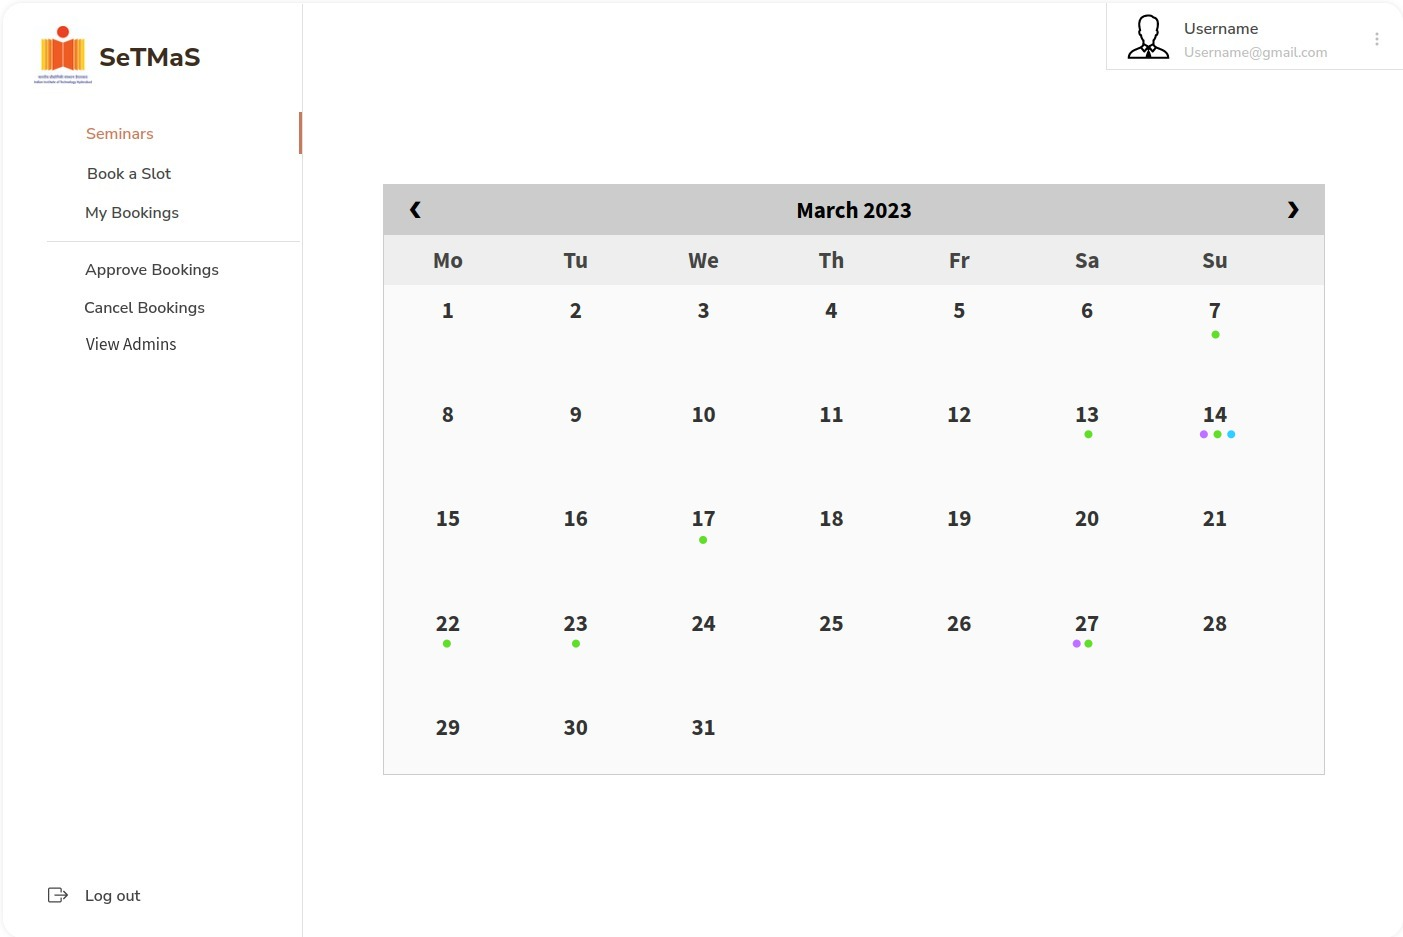
\includegraphics[width=\textwidth]{SeTMaS_HomeScreen_UI.jpeg}
    \caption{Admin Home Page}
    \label{fig:admin_home}
\end{figure}
Above is a potential UI sketch of the home page for a logged-in admin. Clicking on a date opens another view with the list of bookings for that day. Clicking on a booking opens a view with the details of the booking. Similarly 

\end{document}
